\chapter{Resultados}
\label{cap4}



\paragraph{} A partir dos modelos criados na Seção \ref{sub:super_models} e dos parâmetros refinados na Seção \ref{sub:est_simulation}, é possível prosseguir com as simulações finais, que compartilham das seguintes configurações:

\begin{itemize}
    \item 71 \textit{tickers} (Tabela \ref{tab:5})
    \item Período de simulação: 01/04/2020 a 31/12/2021
    \item Capital: R\$ 100000,00
    \item Volume mínimo de ações por negociação: 1
    \item Risco de entrada por operação: 0,29
    \item Período máximo de dias por operação: 45
\end{itemize}

\paragraph{} Observa-se que o período de simulação é posterior ao utilizado para refinamento dos parâmetros de simulação (01/01/2019 a 31/12/2020).

\paragraph{} A Tabela \ref{tab:395} mostra 4 perfis de simulação diferentes, cada um motivado por uma questão diferente, são elas: (1) o máximo local na região de baixo RCC da Figura \ref{fig:550}; (2) o máximo local da região de alto RCC, também da Figura \ref{fig:550}; (3) a simulação de maior índice de Shape da Figura \ref{fig:153} pertencente à curva \begin{math} RCC \times K = 1,8 \end{math}; e (4) a simulação de menor perda de operações na Figura \ref{fig:155}, pertencente à curva \begin{math} RCC \times K = 0,1 \end{math}. Também são apresentados os respectivos resultados.

\begin{table}[!htb]
    \begin{center}
        \resizebox{\textwidth}{!}{
        \begin{tabular}{ l|c|c|c|c|c }
            Parâmetro & Estratégia 1 & Estratégia 2 & Estratégia 3 & Estratégia 4 & \textit{Baseline} \\
            \hline
            RCC     & 0,11\%    & 6,10\%    & 0,00288\% & 0,1\% & - \\
            K       & -         & -         & 62500     & 100   & - \\
            \hline
            Rendimento Final                    & \% & \% & \% & \% & 68,07\% \\
            Volatilidade                        & \% & \% & \% & \% & 34,84\% \\
            Índice de Sharpe                    &  &  &  &  & 1,15 \\
            Índice de Sortino                   &  &  &  &  & 1,71 \\
            Cor. Spearman (\textit{Baseline})   &  &  &  &  & - \\
            Cor. Spearman (Ibovespa)            &  &  &  &  & - \\
            Uso Máximo de Capital               & \% & \% & \% & \% & 100\% \\
            Uso Médio de Capital                & \% & \% & \% & \% & 100\% \\
            Máximo de Op. Ativas                &  &  &  &  & 71 \\
            Média de Op. Ativas                 &  &  &  &  & 71 \\
            % Desvio Padrão de Op. Ativas         &  &  &  &  & - \\
            Operações Totais                    &  &  &  &  & 71 \\
            Operações de Sucesso                &  (\%) &  (\%)&  (\%)&  (\%) & - \\
            Operações de Falha                  &  (\%) &  (\%)&  (\%)&  (\%) & - \\
            Operações de \textit{Timeout}       &  (\%) &  (\%)&  (\%)&  (\%) & - \\
            Operações Incompletas               &  (\%) &  (\%)&  (\%)&  (\%) & - \\
        \end{tabular}}
        \caption{Resultados finais}
        \label{tab:395}
    \end{center}
\end{table}


\paragraph{} Cortar daqui para baixo.




% \paragraph{} A partir dos parâmetros descritos e refinados na Seção \ref{sub:est_simulation}, utilizou-se a seguinte configuração para encontrar a simulação com os melhores índices de performance:

% \begin{itemize}
%     \item 71 \textit{tickers} (Tabela \ref{tab:5})
%     \item Período de simulação: 01/01/2019 a 31/12/2021
%     \item Capital: R\$ 100000,00
%     \item Volume mínimo de ações por negociação: 1
%     \item Risco de entrada por operação: 0,29
%     \item Período máximo de dias por operação: 45
%     \item RCC: 0,000025
%     \item Controle Proporcional para Uso de Capital (RCC Dinâmico): Sim
%     \item Valor de Referência: 100\%
%     \item Constante K de Ganho Proporcional: 30000
% \end{itemize}

% \paragraph{} Conforme descrito na Seção \ref{sub:risk_man}, a escolha dos 71 \textit{tickers} foi realizada levando em consideração as seguintes preferências: diversidade de segmentos de mercado; disponibilidade da série temporal de dados a partir de 2013; e presença na composição do iBovespa em qualquer data. O período de simulação escolhido engloba um intervalo recente dos últimos 3 anos, já que a escolha de momentos anteriores a este pode estar associado a padrões de mercado muito diferentes do atual. Como os modelos criados utilizam \textit{walk-forward analysis} e portanto atualizados a cada 3 meses de simulação para cada \textit{ticker}, o comprimento do intervalo de 3 anos não é um problema. O capital e o volume mínimo por negociação foram escolhidos visando evitar potenciais problemas quanto à granularidade dos montantes de negociação.

% \paragraph{} Os demais parâmetros revelam valores refinados através de suas respectivas seções, a mencionar: Seção \ref{sub:operation_risk} para o Risco de entrada por operação; Seção \ref{sub:max_op_days} para o Período máximo de dias por operação; e Seção \ref{sub:dynamic_rcc} para o RCC, o Valor de referência e a Constante K.

\paragraph{} Os resultados encontrados podem ser verificados pela Figura \ref{fig:250} e pela Tabela \ref{tab:13}.

\begin{figure}[!htb]
    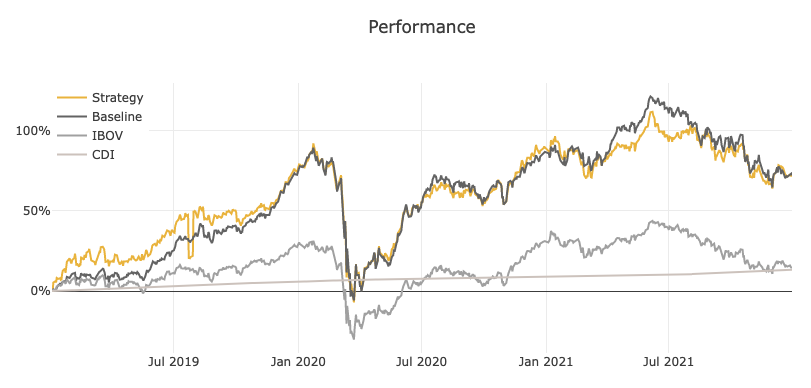
\includegraphics[scale=0.50]{performance_final.png}
    \centering
    \caption{Performance final}
    \label{fig:250}
\end{figure}

\begin{table}[h!] %ID 485
    \begin{center}
        \begin{tabular}{ l|c|c }
            Parâmetro & Estratégia & \textit{Baseline} \\
            \hline
            Rendimento Final & 72,79\% & 73,94\% \\
            Volatilidade & 63,20\% & 55,48\% \\
            Índice de Sharpe & 0,64 & 0,68 \\
            Índice de Sortino & 0,74 & 0,74 \\
            Correlação de Spearman (c/ \textit{Baseline}) & 0,99 & - \\
            Correlação de Spearman (c /Ibovespa) & 0,92 & - \\
            Uso Máximo de Capital & 100\% & 100\% \\
            Uso Médio de Capital & 97,22\% & 100\% \\
            Máximo de Operações Ativas & 71 & - \\
            Média de Operações Ativas & 65,97 & - \\
            Desvio Padrão de Operações Ativas & 6,13 & -\\
            Operações Totais & 3145 & 71 \\
            Operações de Sucesso & 891 (28,3\%) & - \\
            Operações de Falha & 2048 (65,1\%) & - \\
            Operações de \textit{Timeout} & 147 (4,7\%) & - \\
            Operações Incompletas & 59 (1,9\%) & - \\
        \end{tabular}
        \caption{Resultado final}
        \label{tab:13}
    \end{center}
\end{table}

\paragraph{} Deve-se lembar que a estratégia ou o modelo \textit{baseline} é uma representação interna da média de rendimento do mercado para a mesma cesta de ações da estratégia a ser simulada (Seção \ref{sub:baseline}). Com isso em mente, observa-se pela Figura \ref{fig:250} que o rendimento da estratégia final fica em torno do \textit{baseline}, com exceção do primeiro ano de simulação, onde o desempenho é significativamente maior.

\paragraph{} A Tabela \ref{tab:13} também mostra que ambas as estratégias obtiveram resultados bem próximos, em particular a estratégia final teve performance ligeiramente inferior, conforme esperado. Analisando individualmente os resultados, o rendimento da estratégia final está apenas 1,15\% abaixo do \textit{baseline}, o que é relevante, mas não tanto quando se tem em mente que este é apenas o retrato de um dos diversos dias de simulação volátil.

\paragraph{} Apesar dos rendimentos finais equivalentes, não de pode deixar de notar o aumento de volatilidade da estratégia final em 7,72\%, o que prejudica sua qualidade. Contudo, a volatilidade não deve ser analisada isoladamente, mas sim através do índice de Sharpe, que está 0,04 pontos abaixo da referência. Um desvio relevante, porém ainda sutil, mostrando que uma parcela da alta de volatilidade foi compensada por um rendimento médio maior. Já o índice de Sortino está igual em 0,74, mostrando que ambas as estratégias possuem o mesmo grau de confiança quando se analisa a rentabilidade em relação às oscilações de capital abaixo da média.

\paragraph{} Dando sequência à análise, as altas correlações de Spearman mostram uma forte dependência da estratégia em relação ao \textit{baseline} e ao iBovespa, o que pode ser facilmente verificado pela Figura \ref{fig:250}. No entanto, aqui valem algumas ressalvas. Como a correlação de Spearman se baseia apenas nos ranques das funções e não propriamente na magnitude dos valores, é um cenário possível uma estratégia obter uma correlação com o \textit{baseline} muito próxima de 1,0 ao mesmo tempo que um rendimento superior. Isso porque o ganho de capital com cada oscilação positiva seria maior do que a perda em uma oscilação negativa. Por outro lado, também é possível um cenário onde uma estratégia com uma baixa correlação de Spearman com o \textit{baseline} apresente um rendimento superior. Este caso em particular seria um caminho mais interessante, pois mostraria uma versatilidade maior da estratégia criada para diferentes tipos de cenários de mercado.

\paragraph{} O uso máximo de capital em 100\% indica apenas que em algum momento todo capital esteve alocado em ativos. Contudo, o uso médio de capital em 97,22\% traz a informação de que como quase todo capital esteve alocado o tempo todo, há pouco espaço para uma melhora de performance de maneira indiscrimidada daqui para frente. Em outras palavras, as melhoras de rendimento precisarão passar por um aprimoramento dos modelos no que diz respeito a quais operações abrir mão para que outras possam prosperar mais. Nota-se que um uso médio de capital em 100\% não seria vantajoso, uma vez que diminuiria-se a disponibilidade de capital para aporte em novas operações. Por outro lado, um uso médio muito baixo indicaria que a estratégia estaria longe de alcançar o seu máximo potencial de performance. Portanto, uma pequena folga é importante e necessária.

\paragraph{} Assim como o uso médio de capital está alto, a média de operações ativas também está, o que é esperado. O mesmo raciocício vale para o máximo de operações ativas e o uso máximo de capital. \color{red} HERALDO: Não mencionei o Desvio Padrão de Operações Ativas por não achar relevante. Devo removê-lo da tabela? Ou deixo assim mesmo? \color{black}

\paragraph{} Por fim, deve-se ressaltar que o número total de operações de 3145 está saturado, conforme explicado ao final da Seção \ref{sub:dynamic_rcc}. Resumidamente, os parâmetros de simulação, em especial o RCC e o K, estão configurados de forma a estressar a estratégia a ponto dela desobedecer em alguns momentos as ordens de compra vindas dos modelos de ML por falta de capital disponível. Tal abordagem trouxe um aumento de performance, mas deve ser usada com cautela. Independentemente desta questão, a taxa de acerto de 28,3\% contra os 65,1\% de falha mostra que apesar da estratégia acertar pouco, o lucro obtido é proporcionalmente maior que as perdas acumuladas.